\subsection{19 августа. Д.р. Кичкинакол Уллукёльский}
\textit{Метеоусловия: утром, днём, вечером ясно, тепло.}

\begin{figure}[h!]
	\centering
	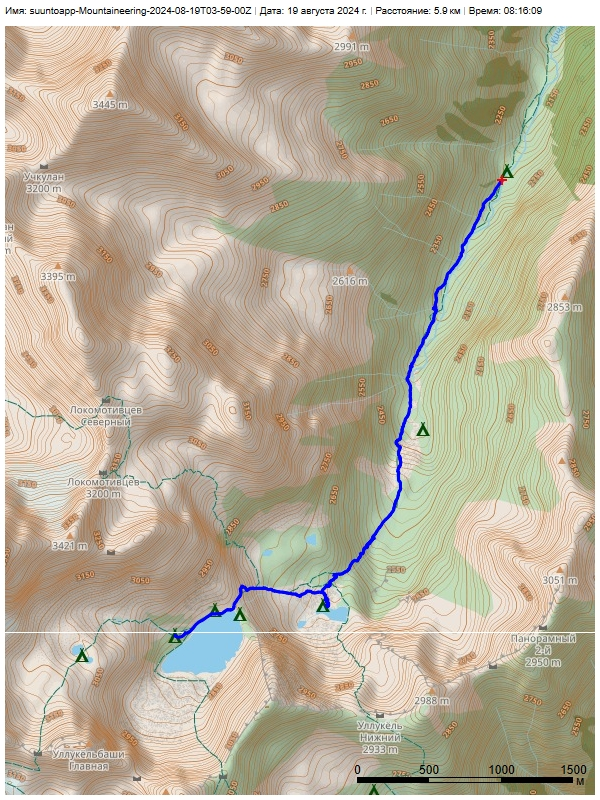
\includegraphics[angle=0, width=0.7\linewidth]{../pics/mini_maps/19}
	\label{fig:mini_19}
\end{figure}

Подъём дежурных в 05:00, общий подъём в 05:30 \remove{под бодрую еврейскую песню на гуслях <<Ломирр зих ибербетн>>.~ }
Выходим в 07:30, идём по левому берегу р. Кичкинакол Уллукёльский по хорошо набитой тропе, попутно  пересекаем старые короткие участки курумника и небольшие притоки реки. В 08:30 выходим на старое моренное плато (рис. \ref{fig:DSC_0692}).

\begin{figure}[h!]
	\centering
	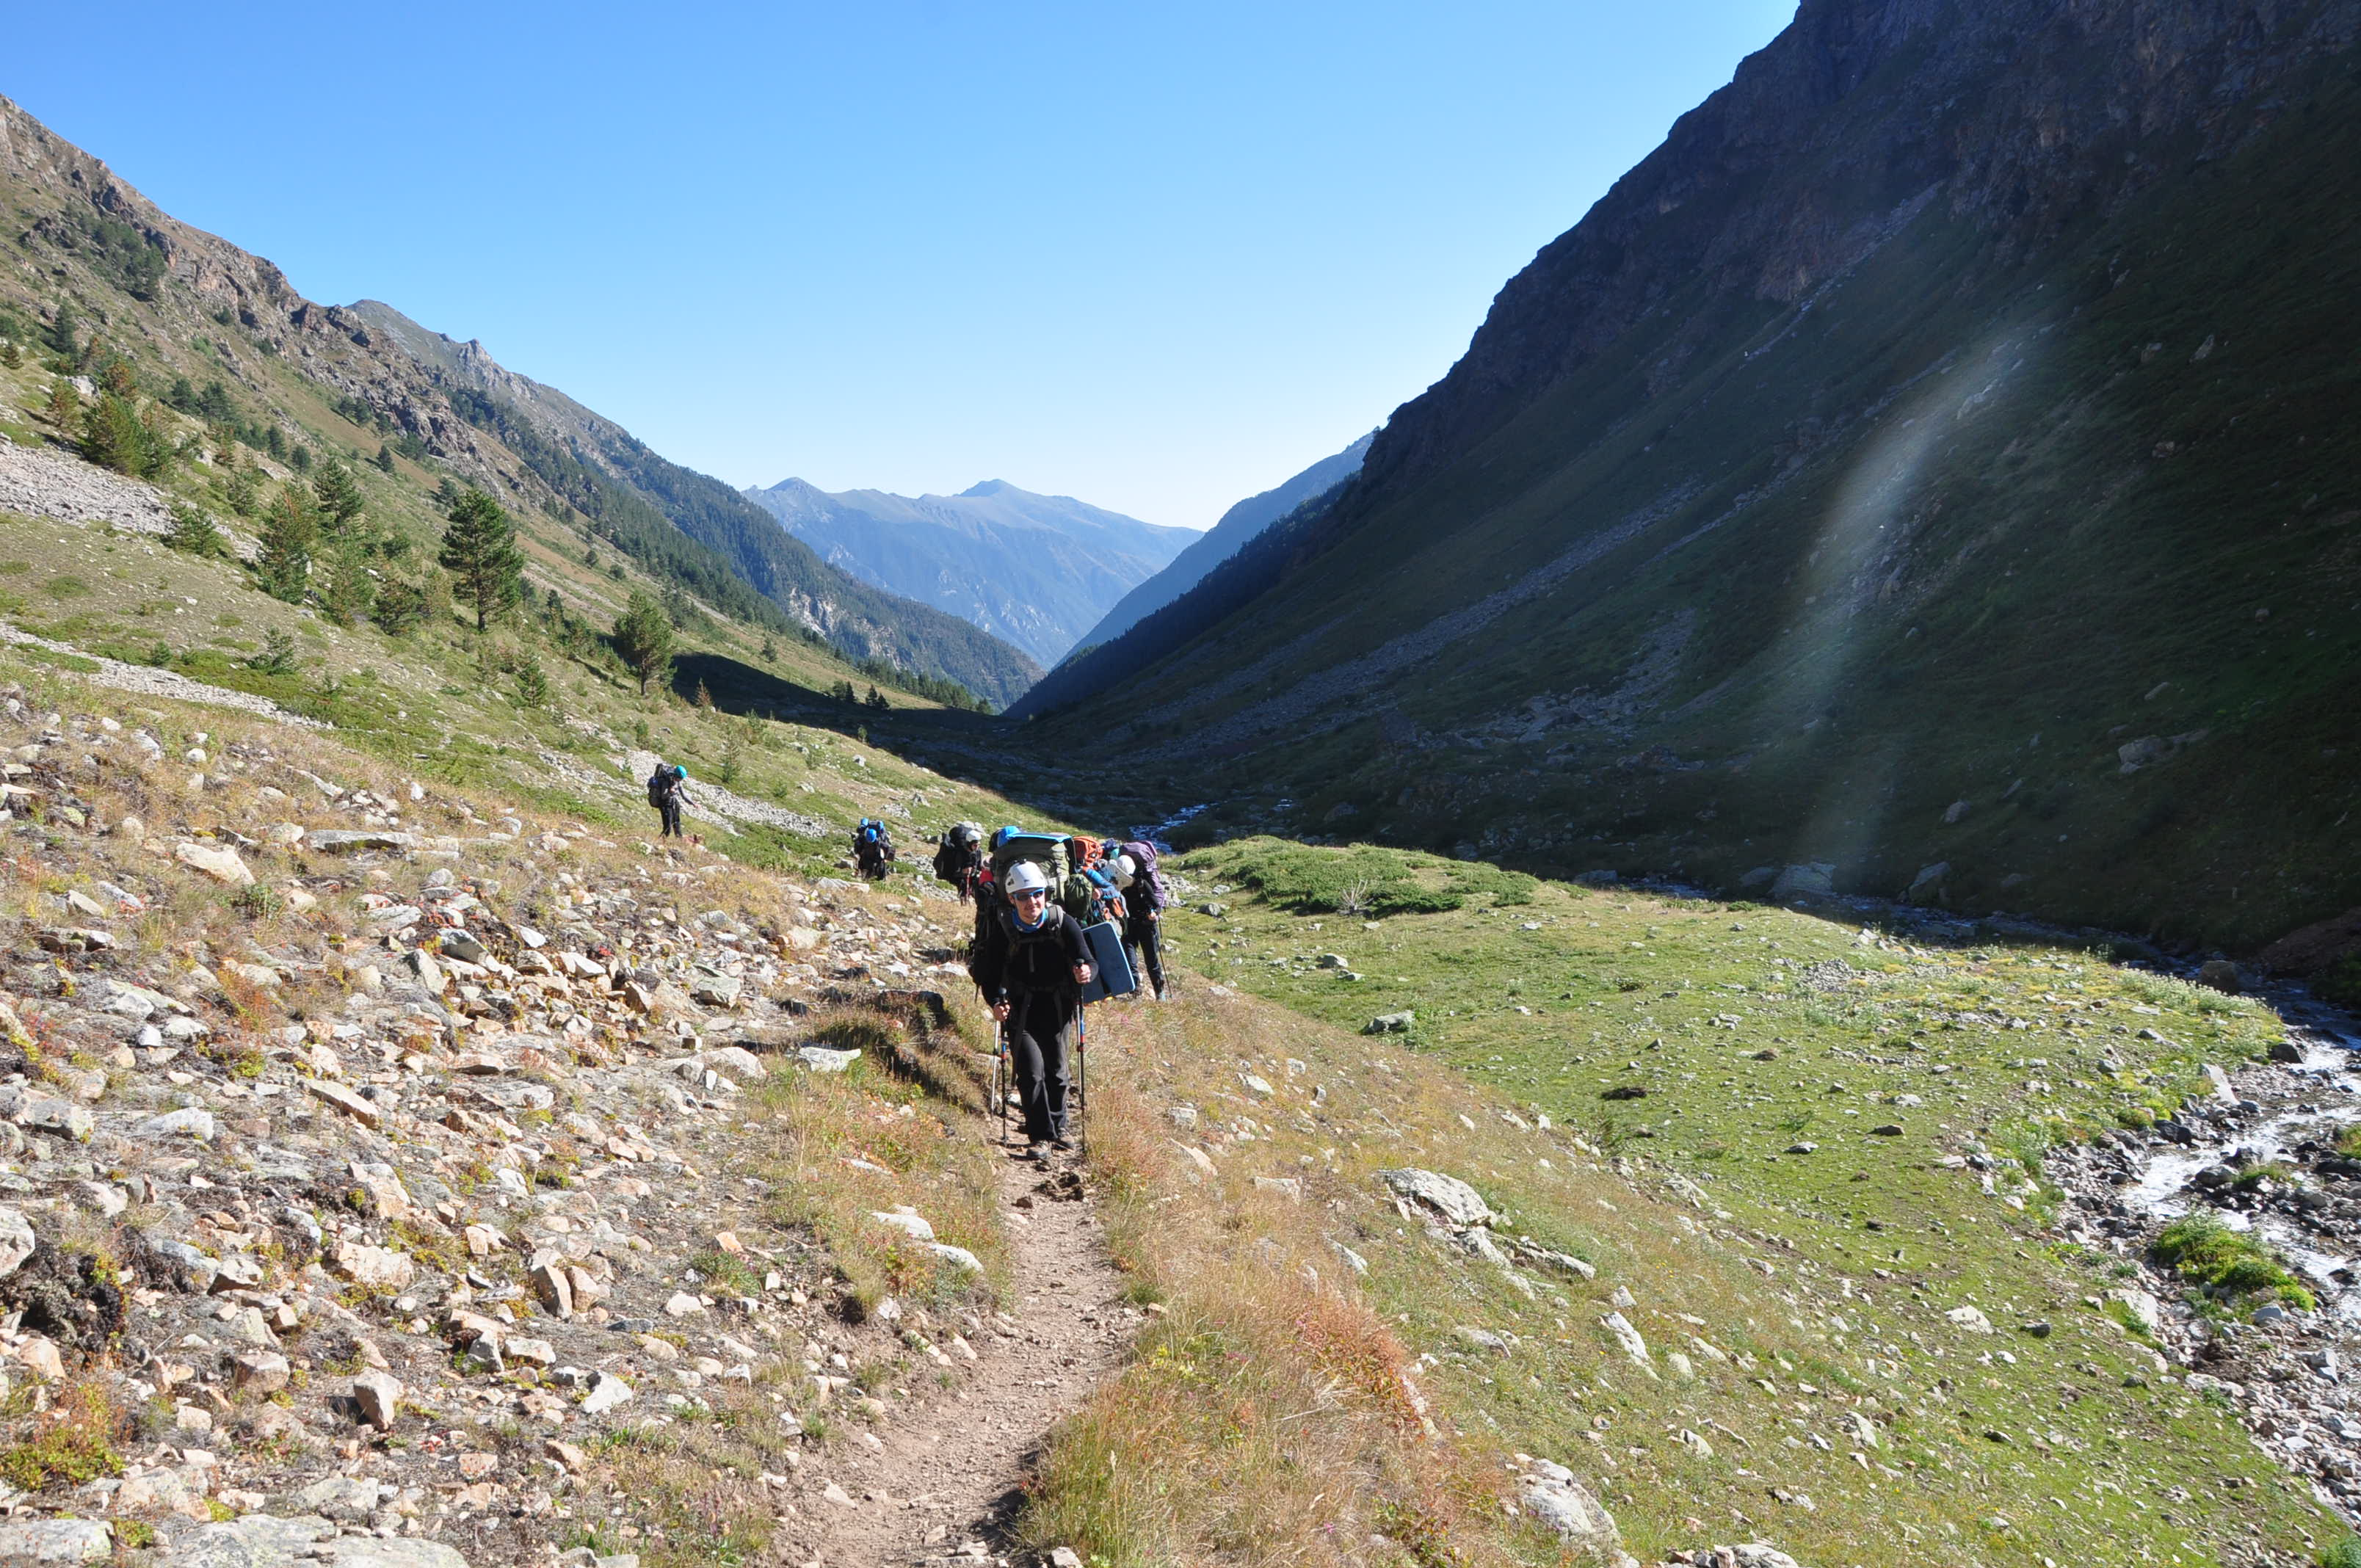
\includegraphics[width=0.7\linewidth]{../pics/DSC_0692}
	\caption{Группа в верховьях д.р. Кичкинакол Уллукёльский}
	\label{fig:DSC_0692}
\end{figure}

Путь от плато к оз. Гитче-Кёль идёт как по левому, так и по правому орогр. берегам р. Кичкинакол Уллукёльский. Мы выбираем первый вариант в силу большей его распространённости и маркированности турами. 

\begin{figure}[h!]
	\centering
	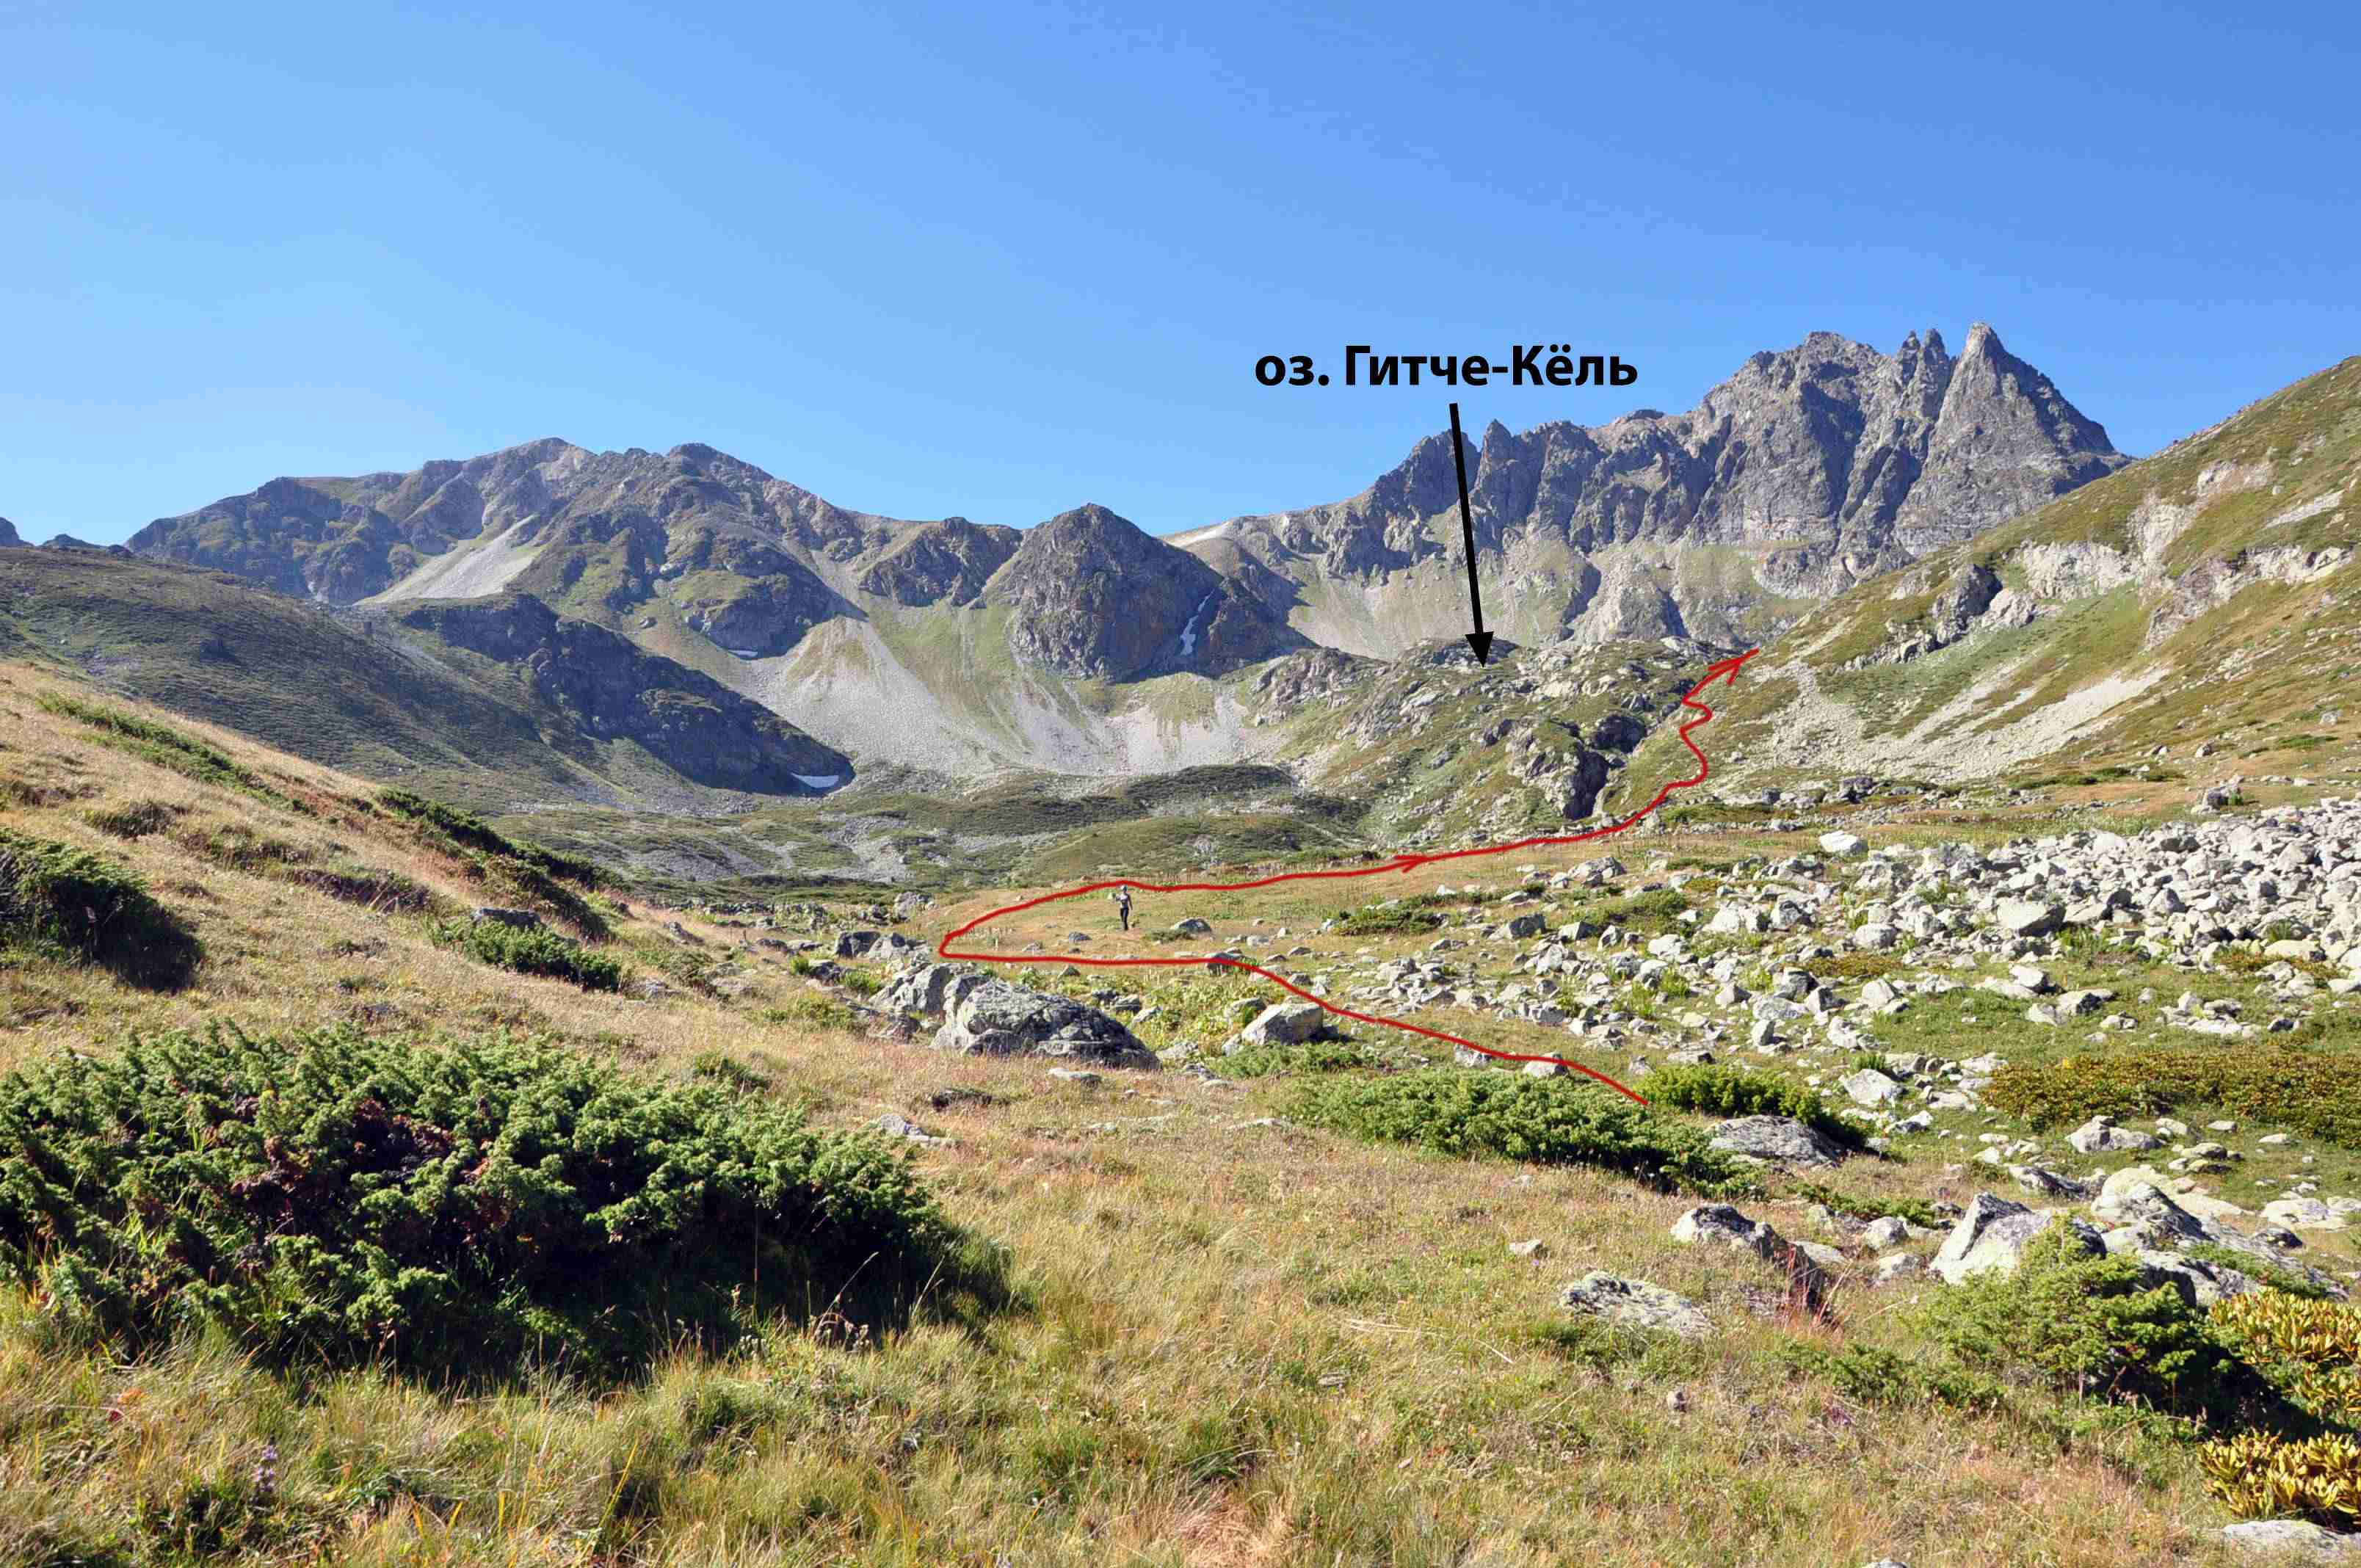
\includegraphics[width=0.7\linewidth]{../pics/DSC_0718}
	\caption{Путь подъёма к оз. Гитче-Кёль}
	\label{fig:DSC_0718}
\end{figure}

Преодолев моренную дамбу крутизной до 25\degree и высотой до 90 м, в 11:15 выходим к оз. Гитче-Кёль (ЧХВ=\alert{СКОЛЬКО?}) и становимся на обед. 
Погода стоит жаркая, мы не спеша готовим обед, купаемся и окончательно решаем идти по основному маршруту на пер. Уллу-Кёль Восточный, а не на пер. Уллу-Кёль Нижний.



\begin{figure}[h!]
	\centering
	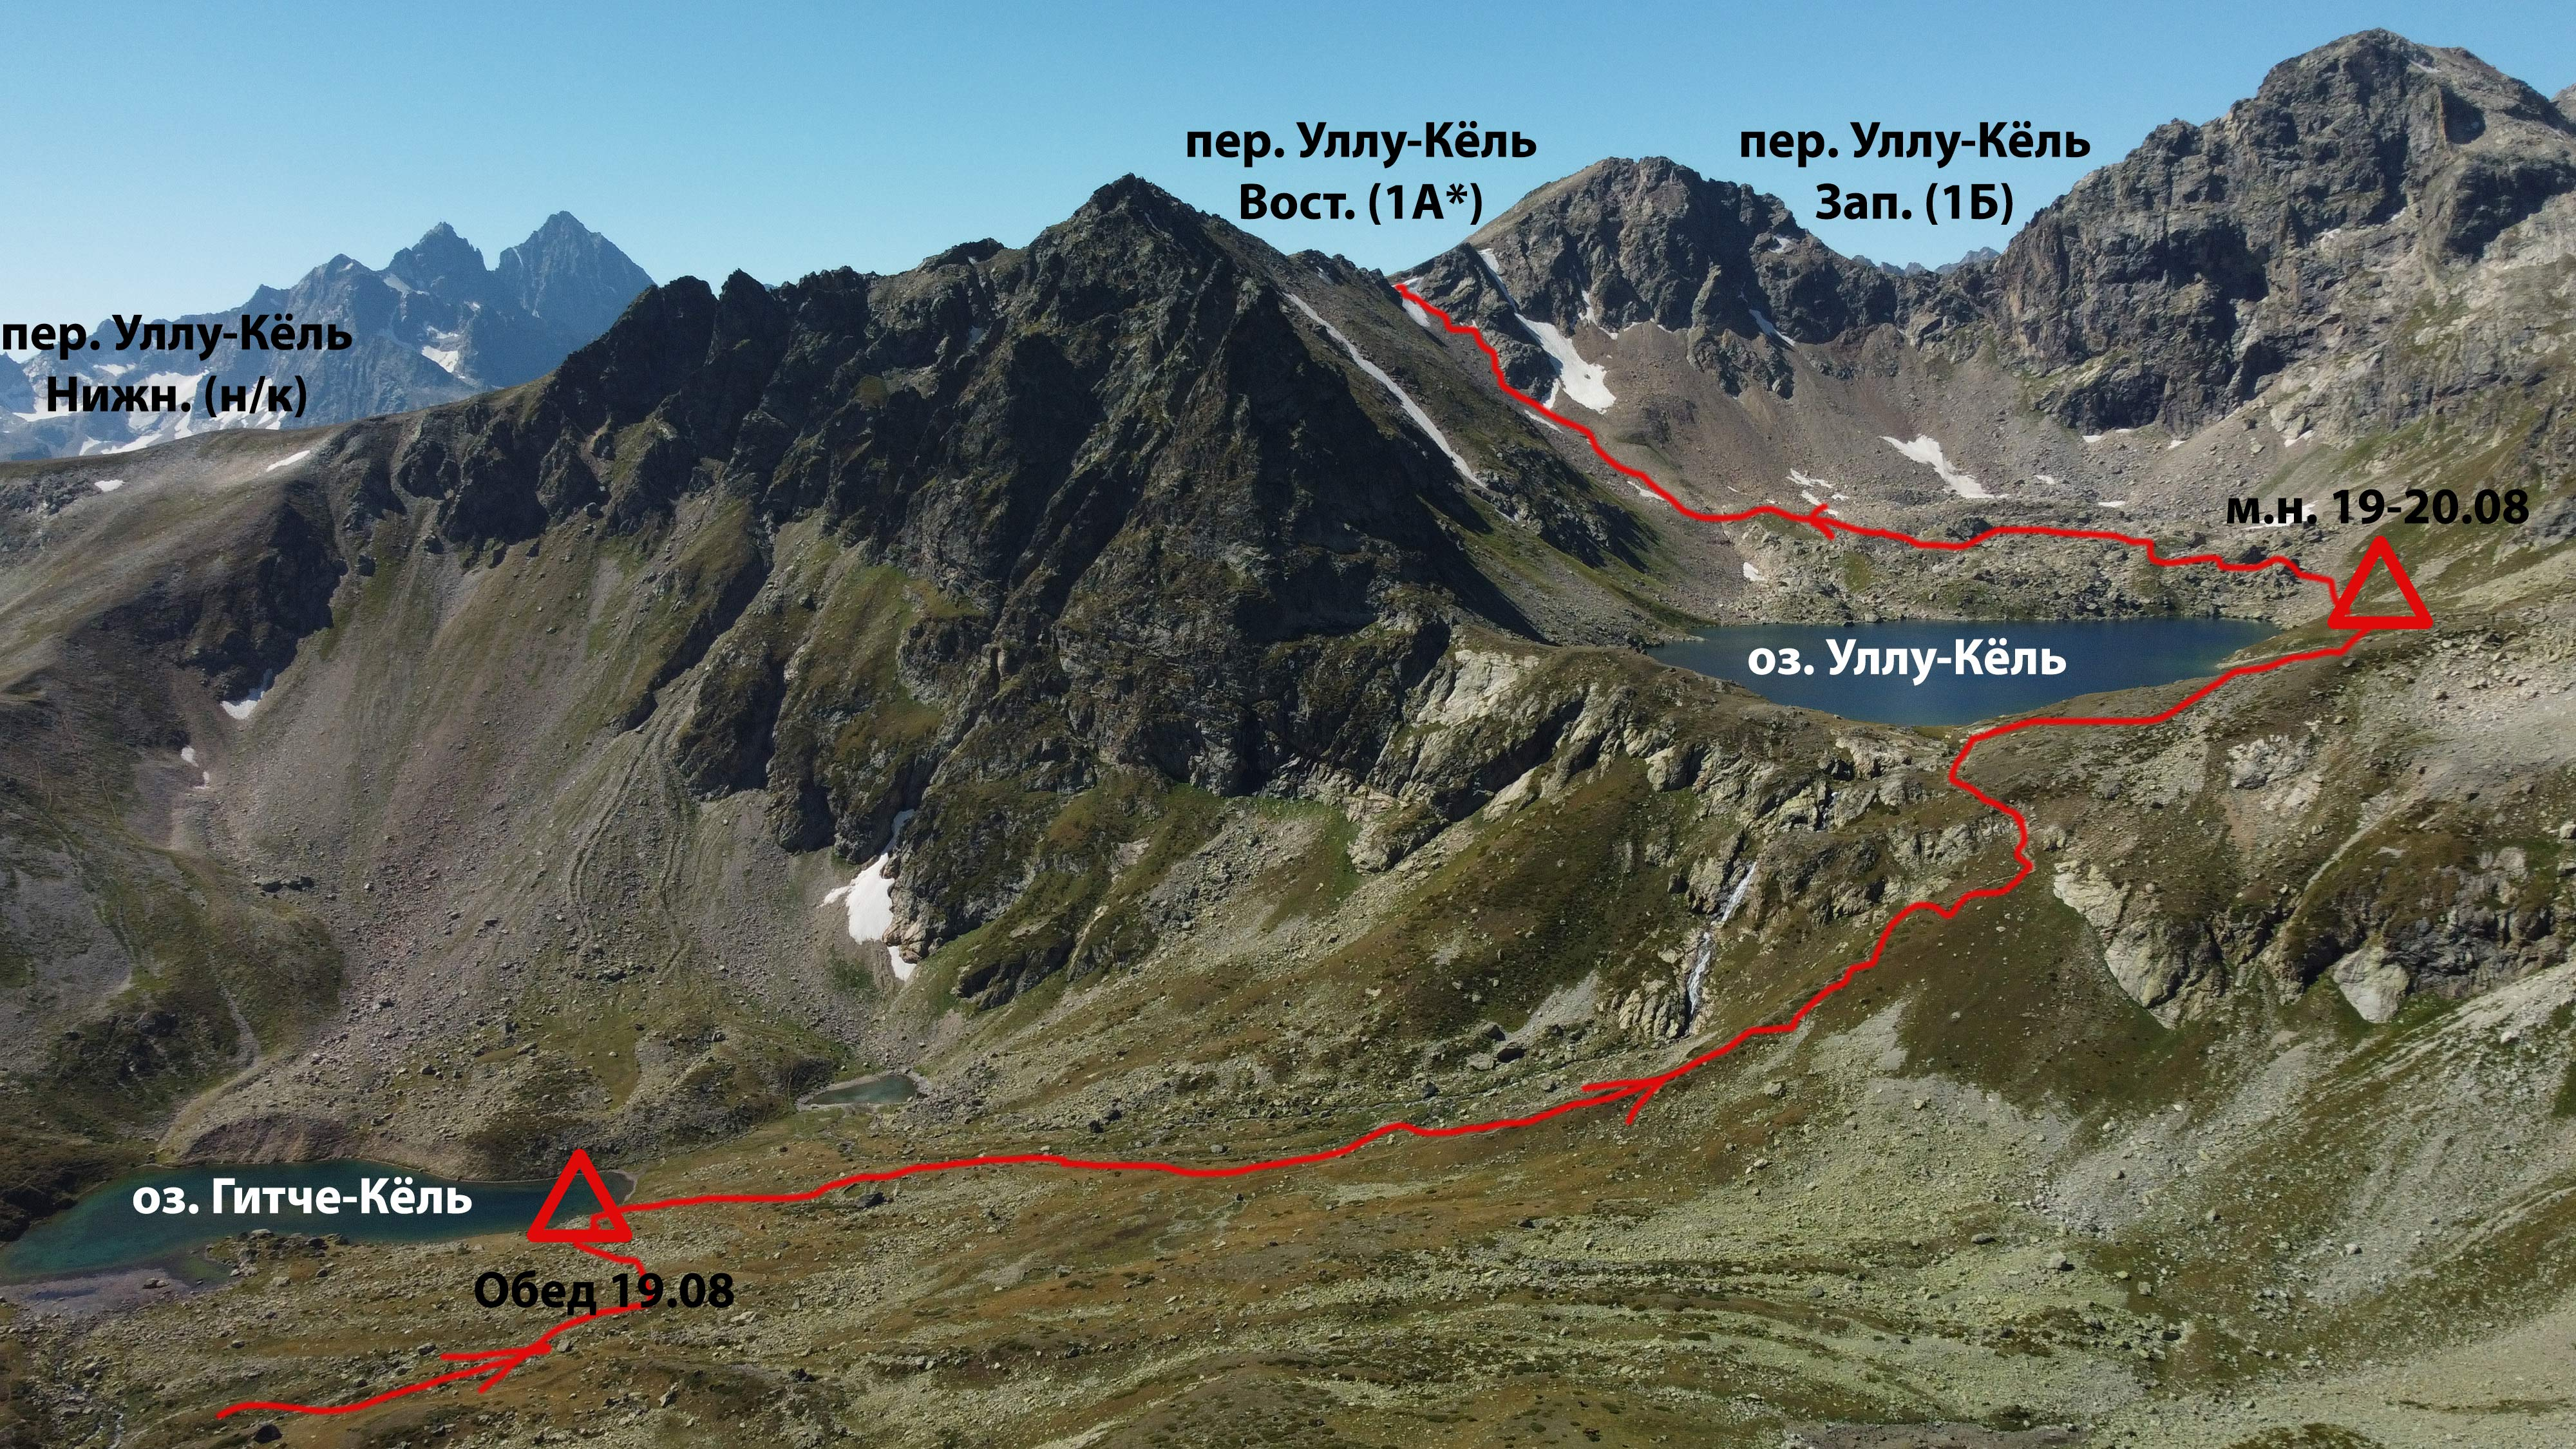
\includegraphics[width=0.7\linewidth]{../pics/ullu_kuel_route}
	\caption{Дорога до озёр и далее на перевал}
	\label{fig:ullu_kuel_route}
\end{figure}

\begin{figure}[h!]
	\centering
	\begin{turn}{0}
		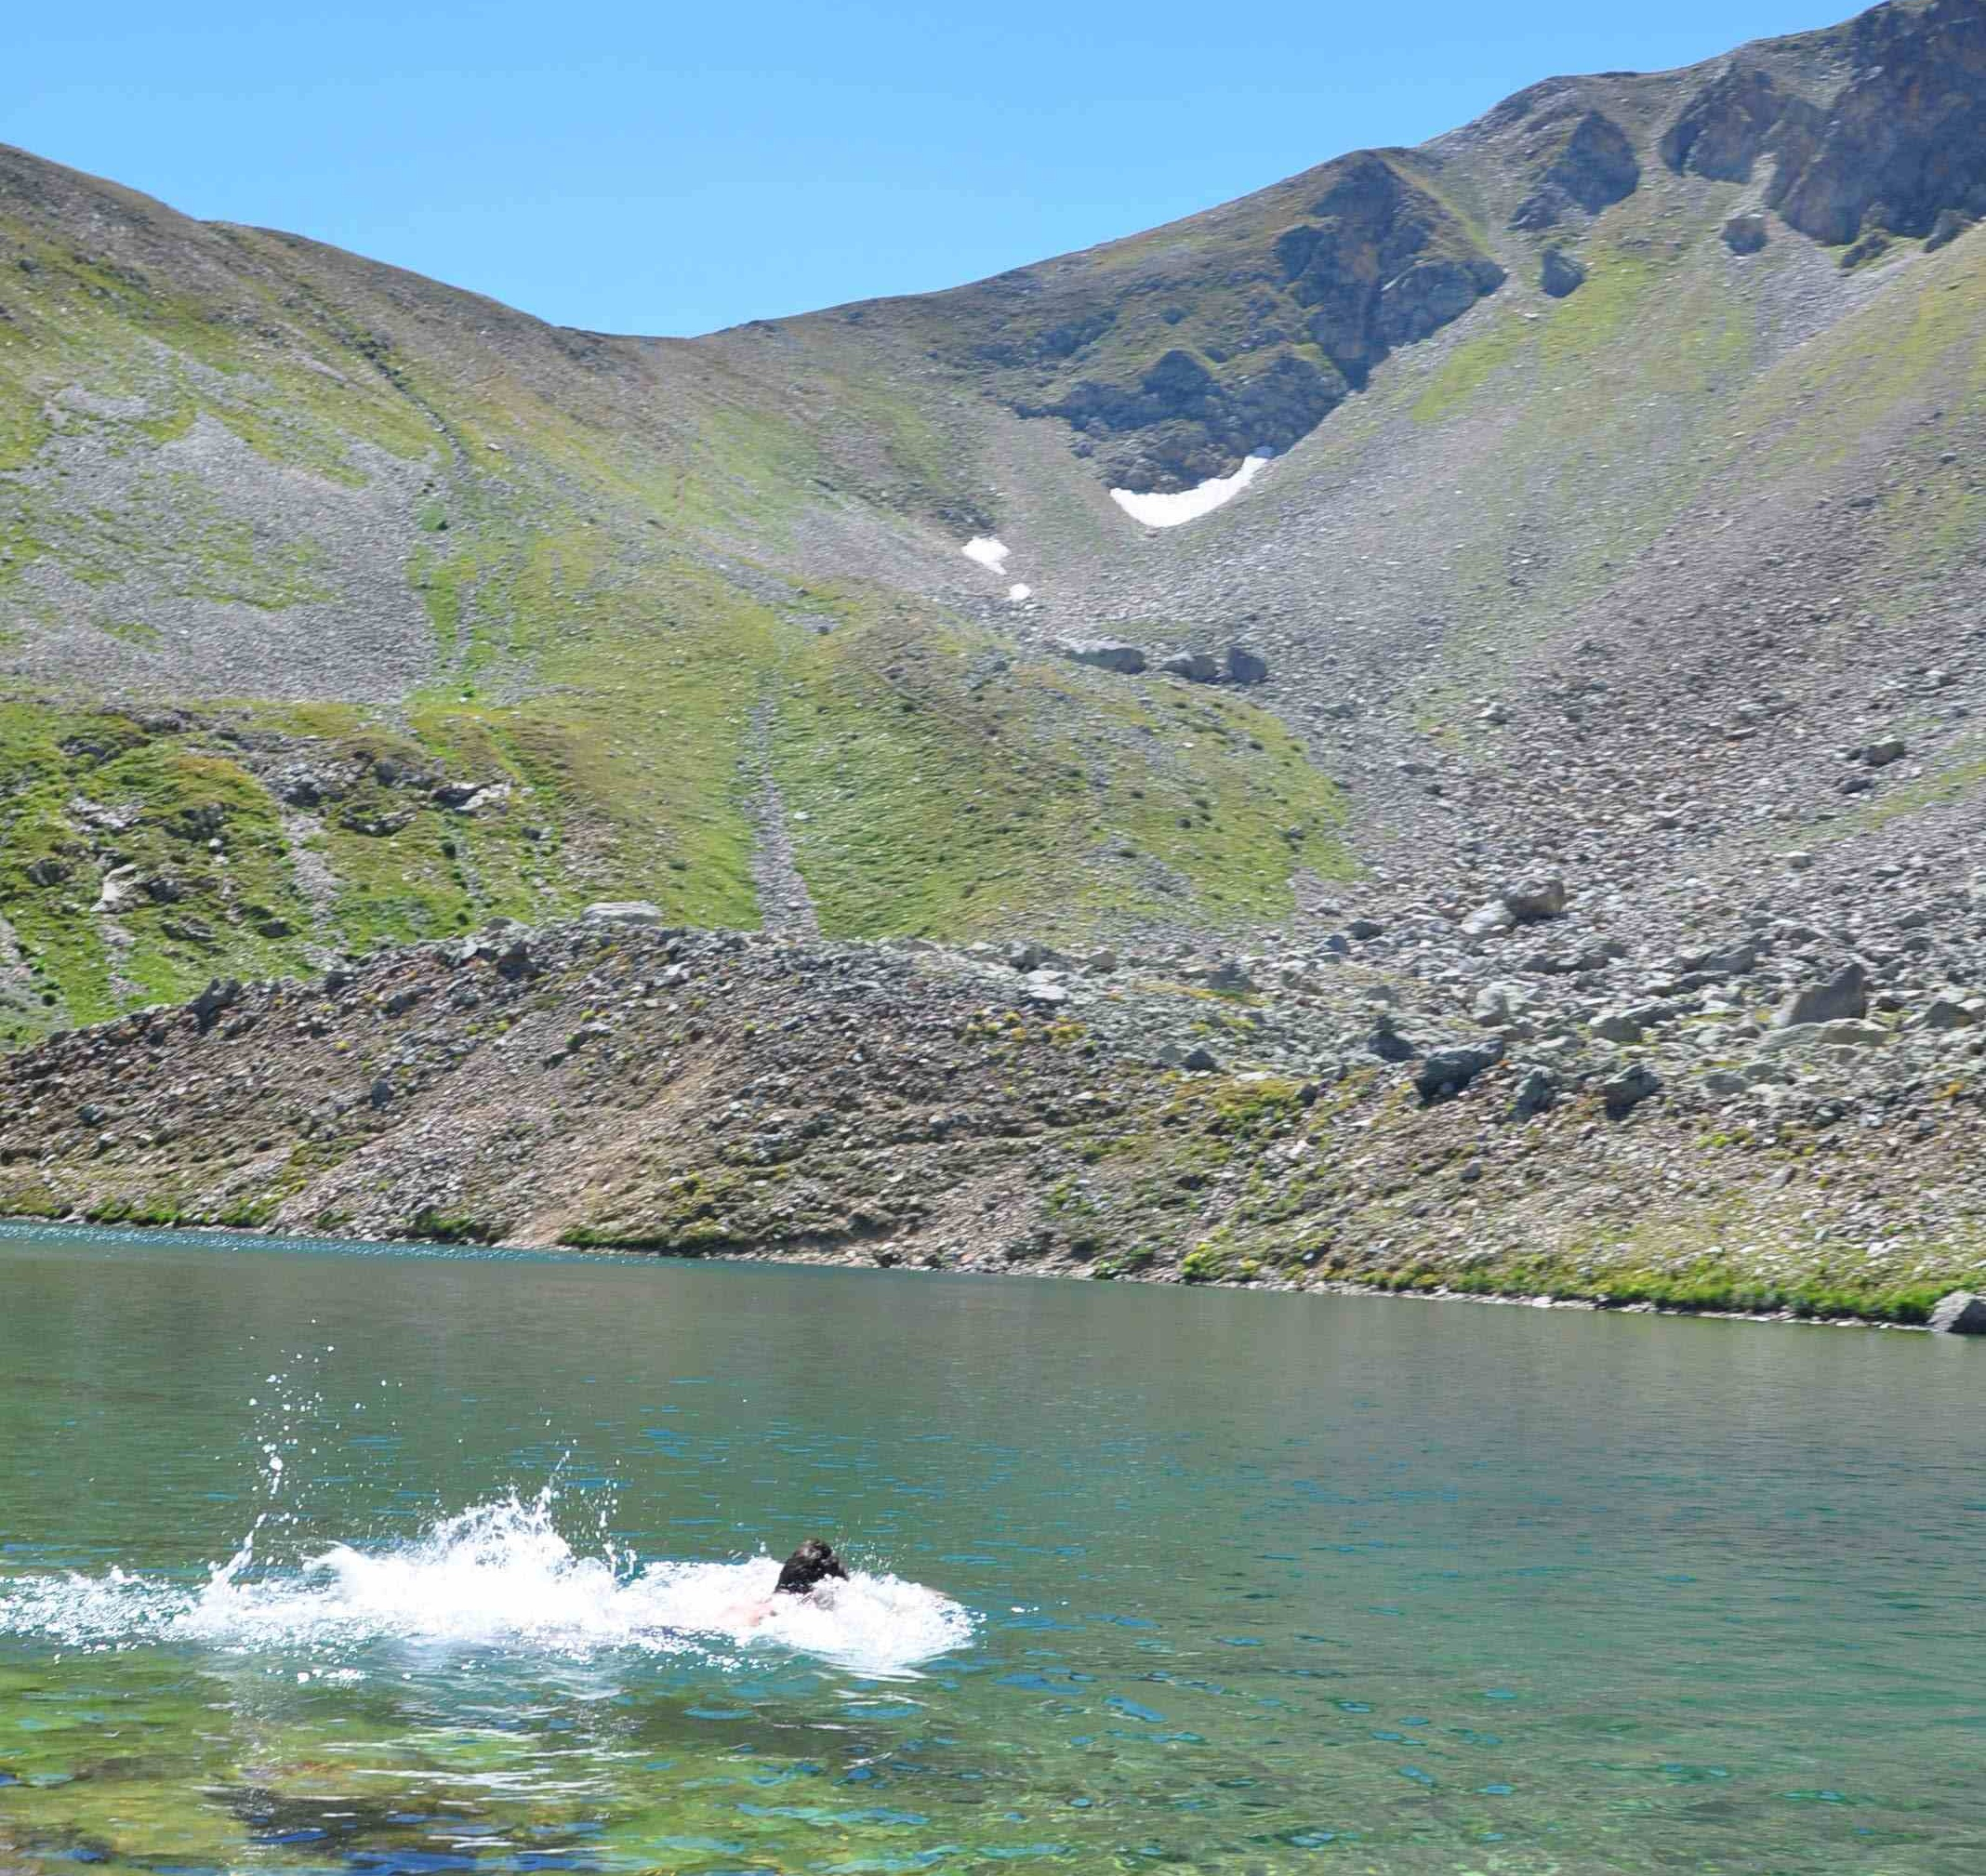
\includegraphics[width=0.7\linewidth]{../pics/DSC_0774}
	\end{turn}
	\caption{Купаемся в оз. Гитче-Кёль}
	\label{fig:DSC_0774}
\end{figure}

К 15:00 выходим на северо-восточную оконечность озера, а в 15:15 становимся на ночёвку на оборудованной стоянке, координаты м.н. N 43.32501\degree E 41.94003\degree

\begin{figure}[h!]
	\centering
	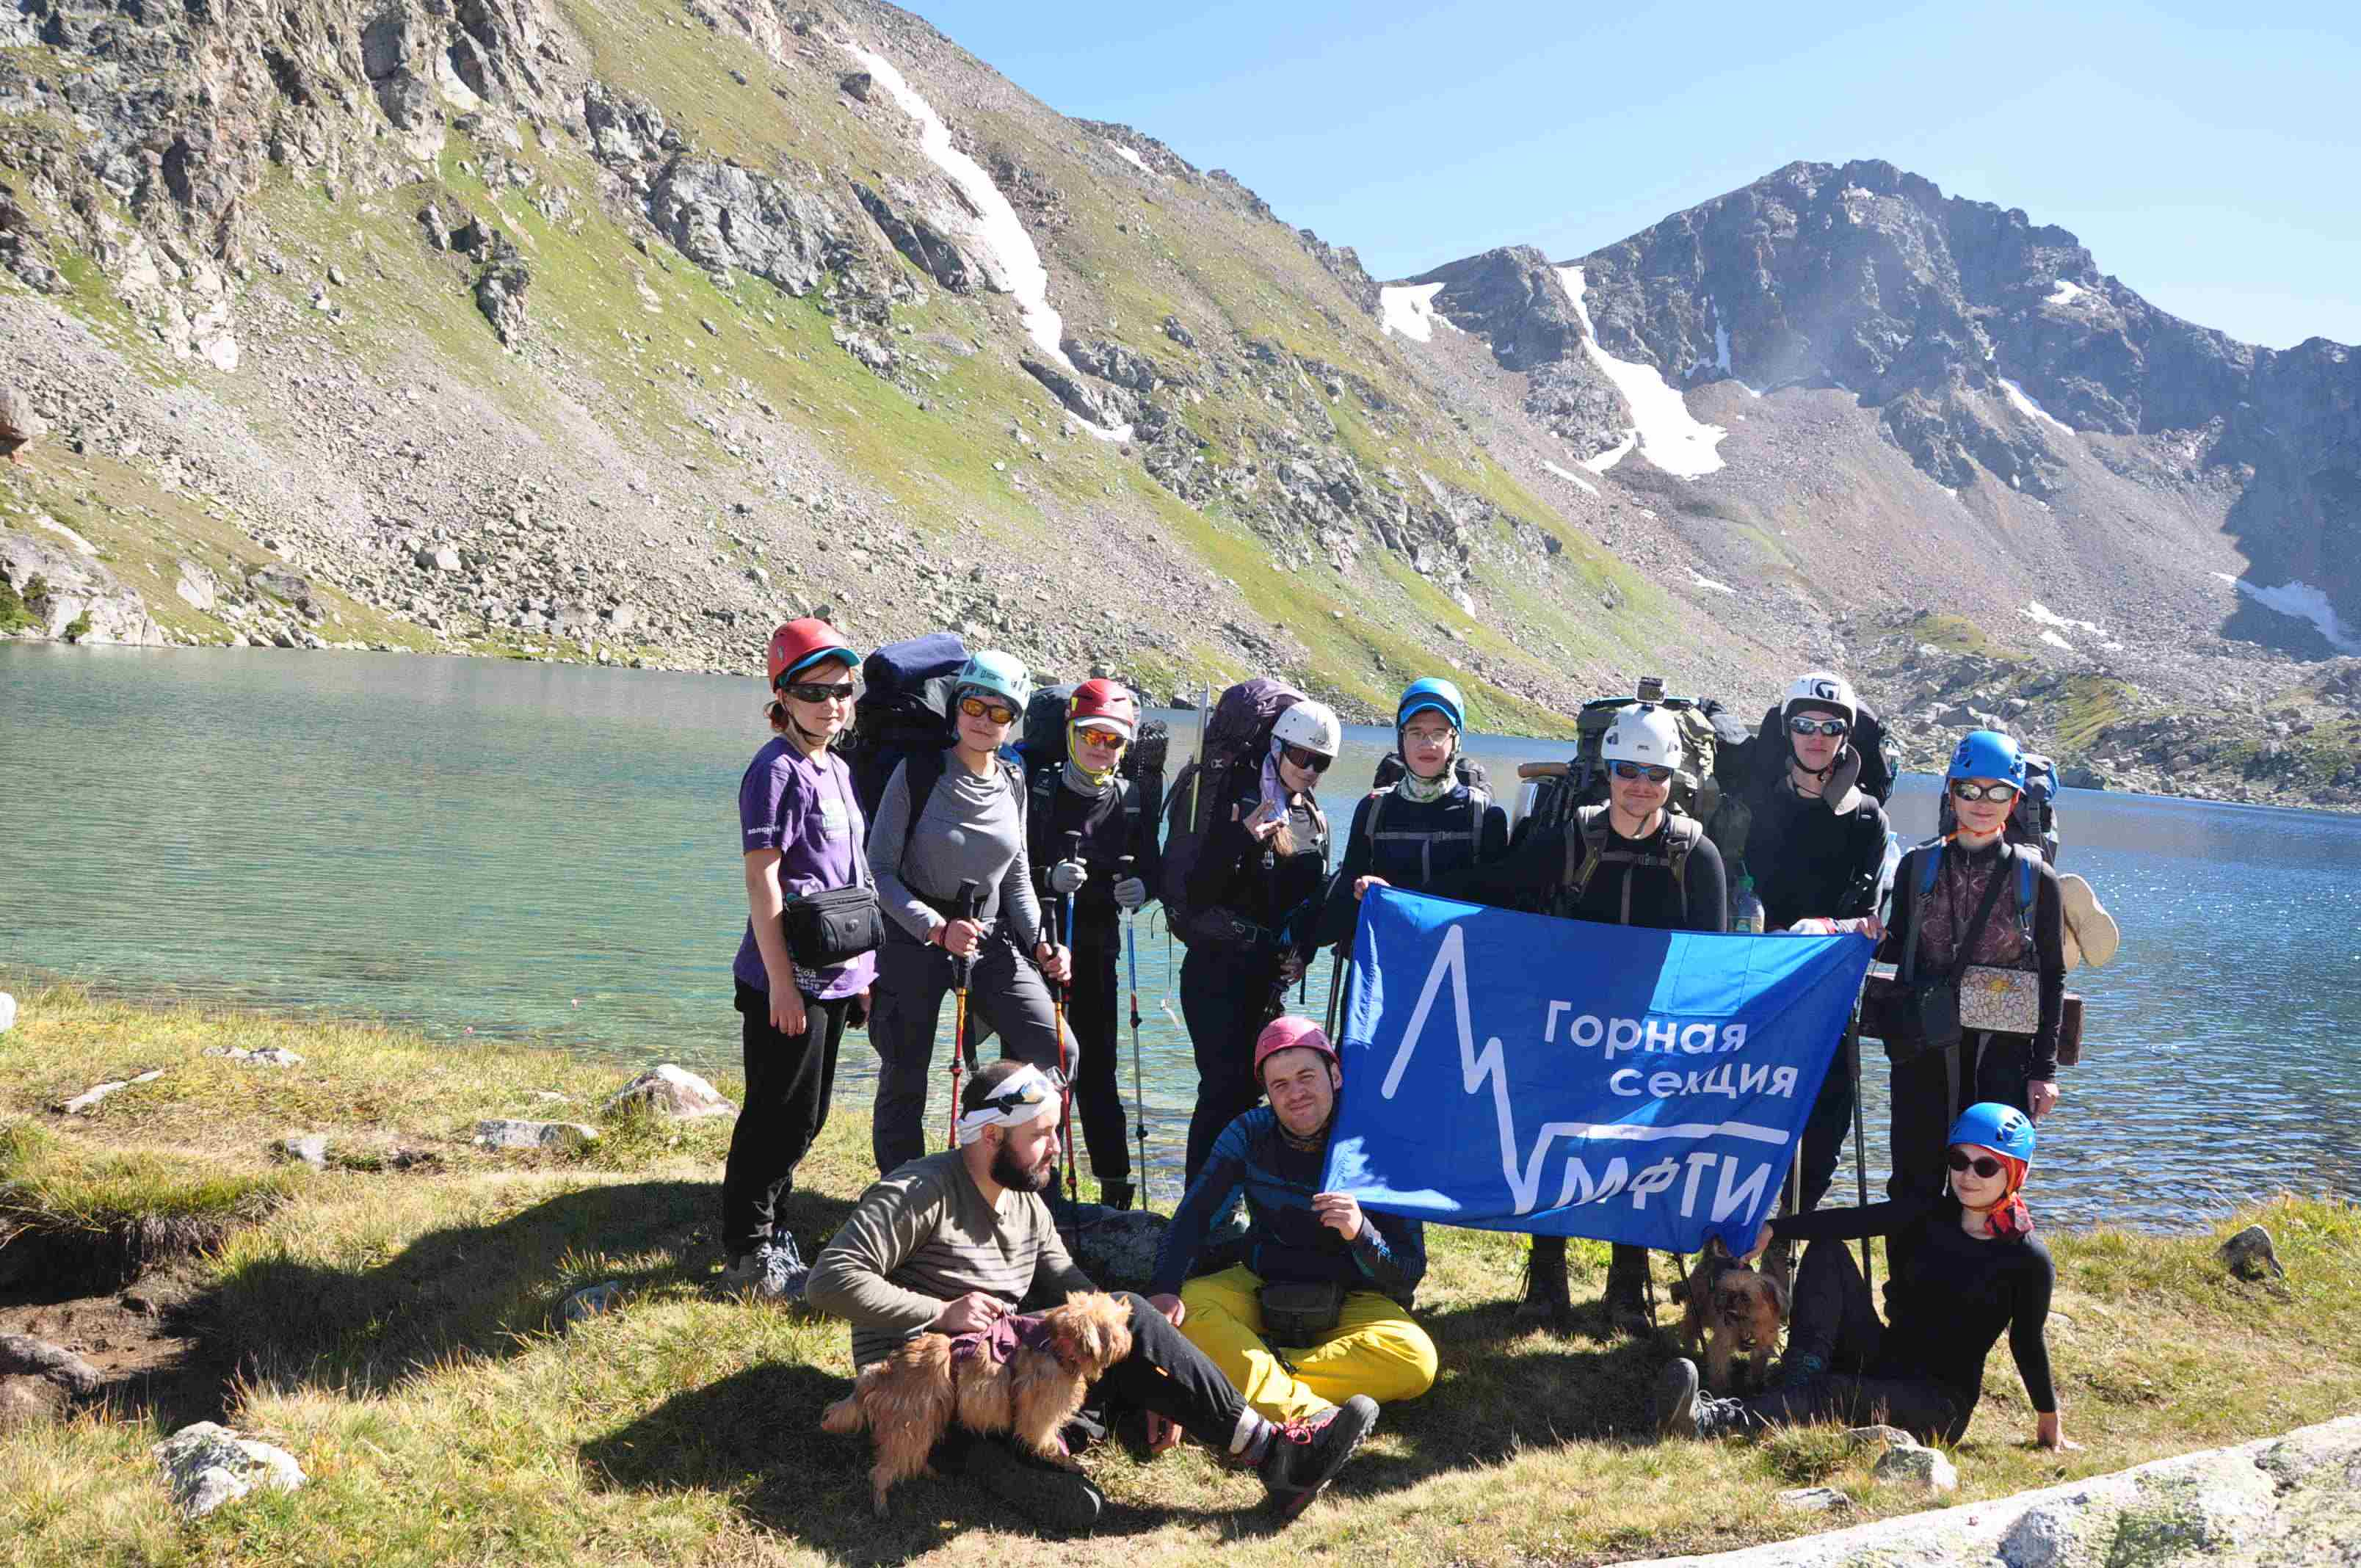
\includegraphics[width=0.7\linewidth]{../pics/DSC_0800}
	\caption{Группа на оз. Уллу-Кёль}
	\label{fig:DSC_0800}
\end{figure}


По случаю полуднёвки решаем провести тренировку по хождению в кошках и самозарубанию на снежном склоне, и в 16:10 выходим из лагеря налегке, треверсируя склон выше крупной осыпи, в направлении снежника под пер. Дырявый (1Б). Траверсируемый склон сначала осыпной, далее травянисто-осыпной крутихной до 25\degree. Такая форма рельева участникам в новинку, и, как следствие, идем мы медленно. Оценив время на тренировку и возвращение, решаем дойти до более близкого пологого снежника, отказаться от тренировки самозарубания и только походить в кошках. Сама тренировка занимает около 30 минут. В некоторый момент мимо нас проходит целое семейство горных козлов в количестве 6 штук.
На обратном пути идём вдоль кромки озера, попутно разведывая завтрашний путь к перевалу.

В лагерь возвращаемся в 17:50, перед сном устраиваем небольшую фотосессию по случаю красивого звёздного неба и яркой луны (рис. \ref{fig:IMG_20240829_194851}).

\begin{figure}[h!]
	\centering
	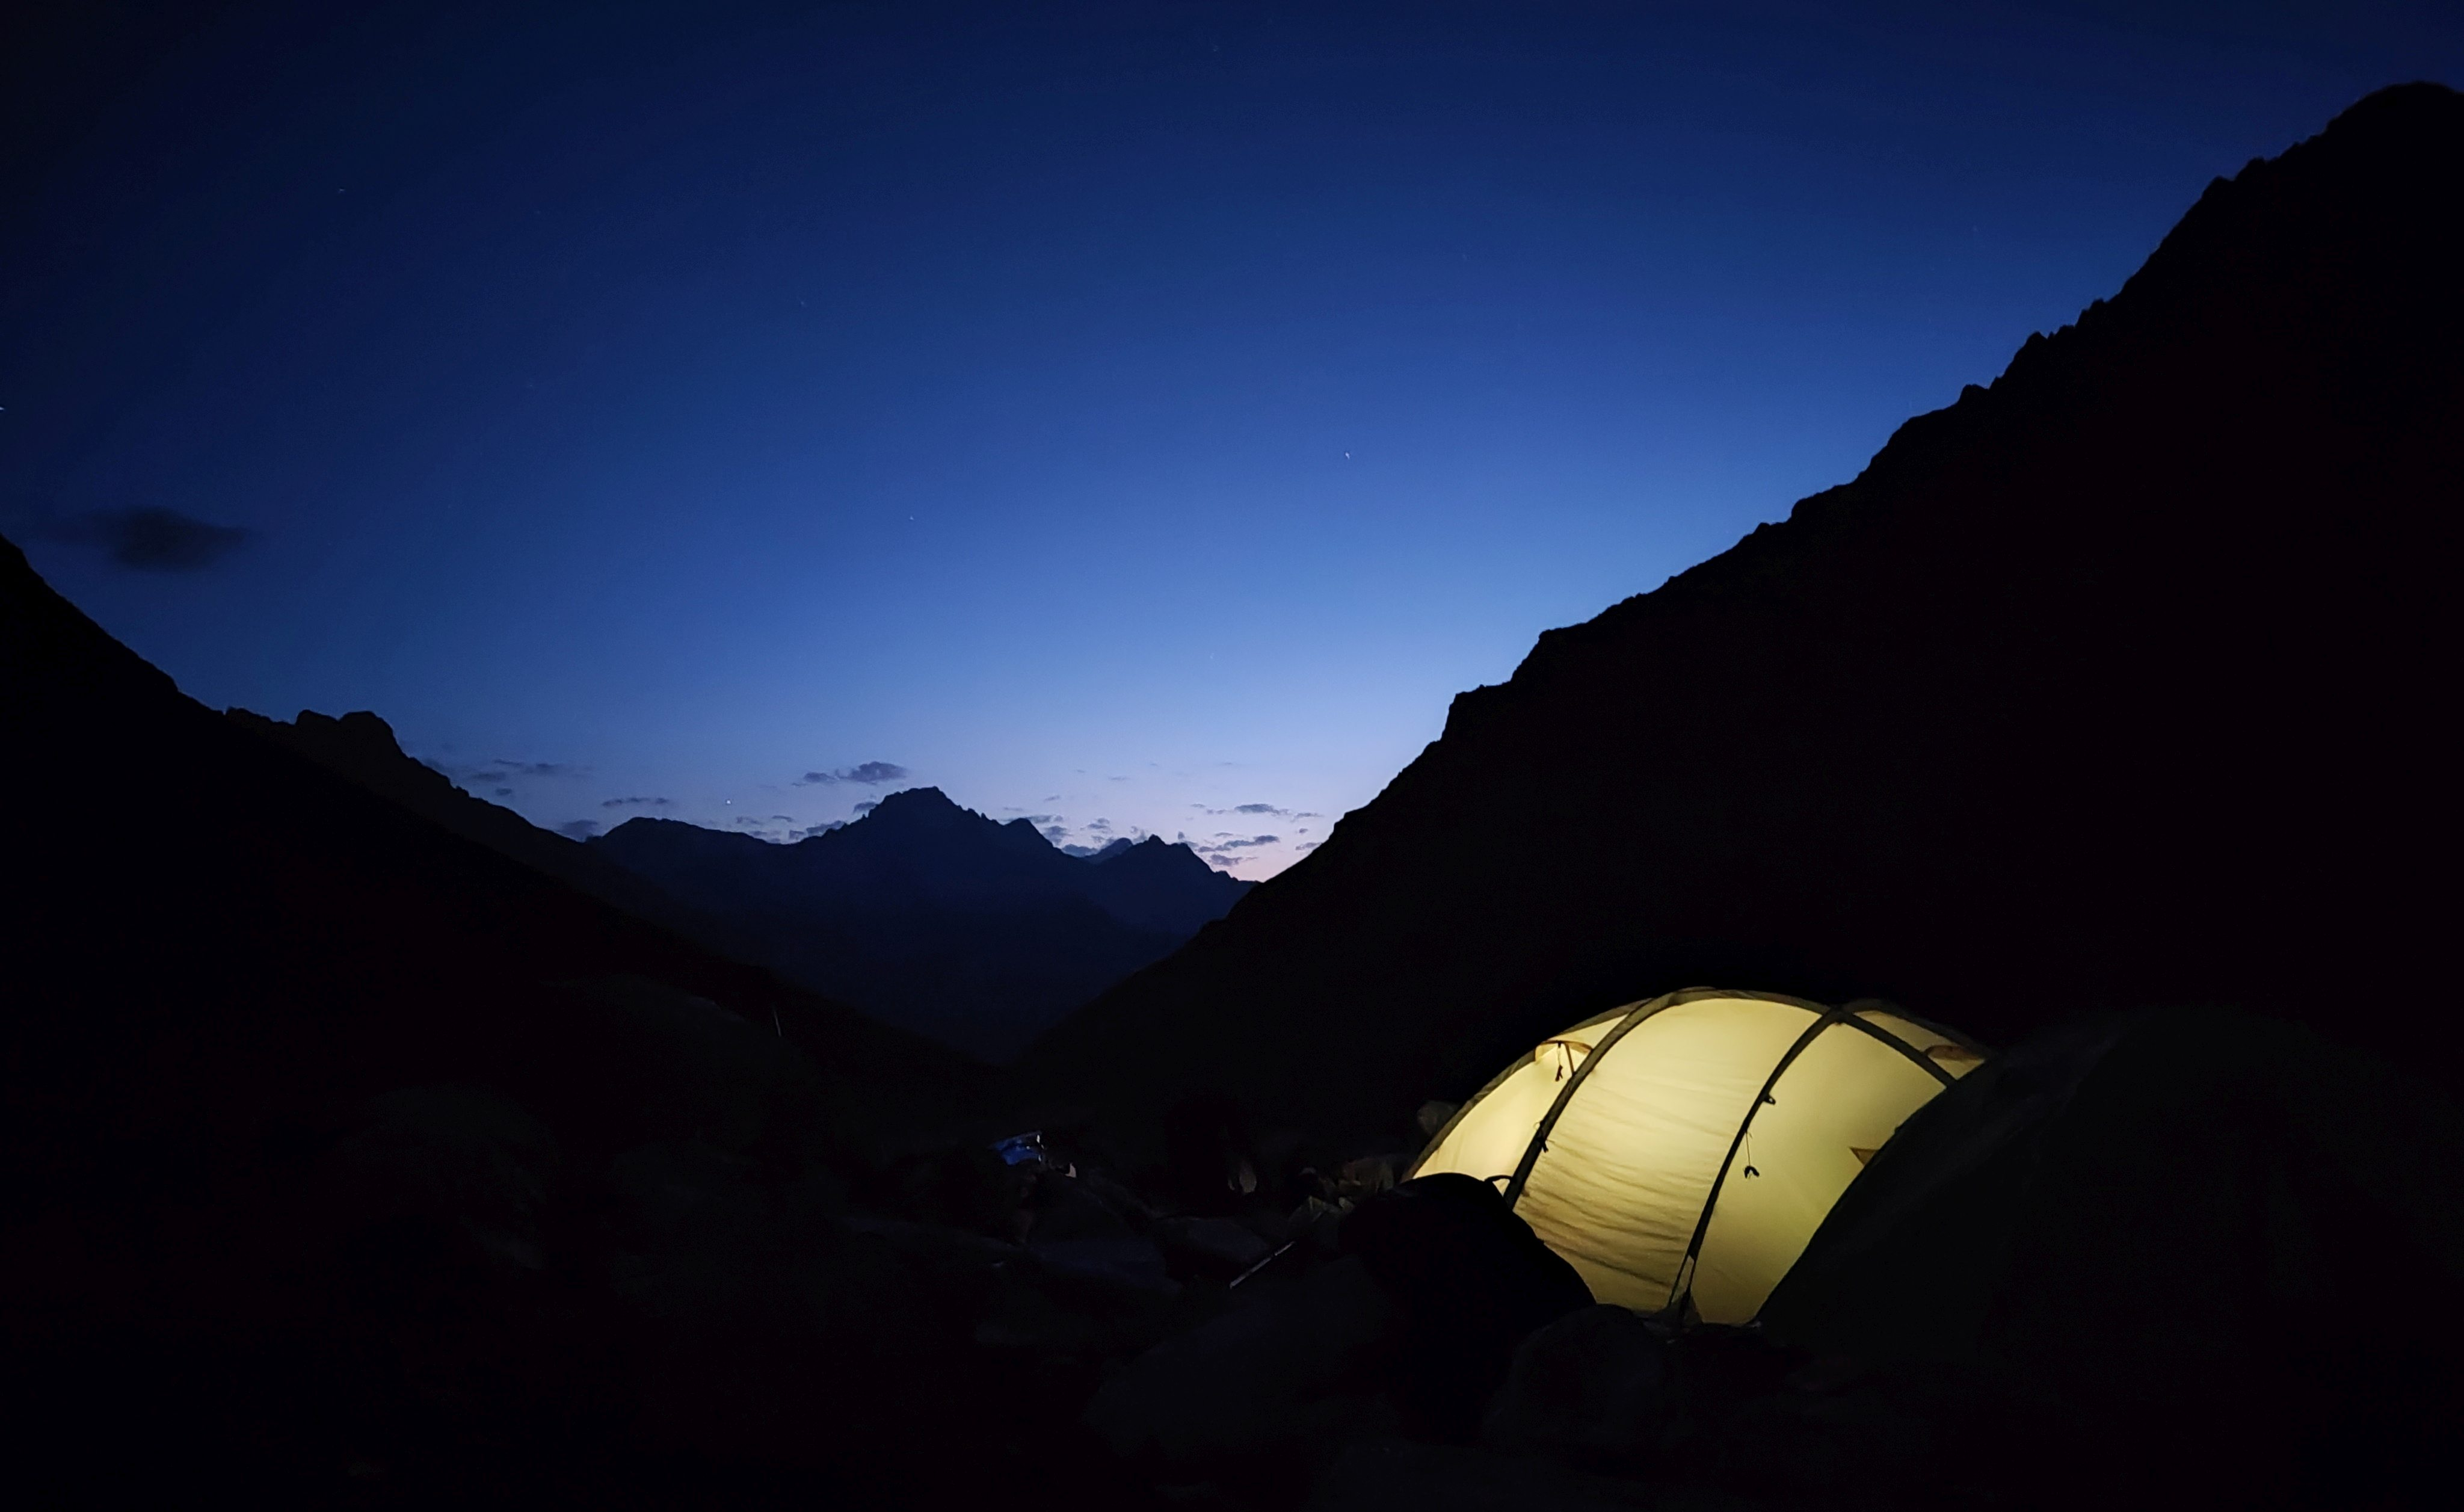
\includegraphics[width=0.7\linewidth]{../pics/IMG_20240829_194851}
	\caption{Место ночёвки 19-20.08}
	\label{fig:IMG_20240829_194851}
\end{figure}

\newpage